\documentclass{article}
\usepackage[left=2cm, right=2cm, top=0cm]{geometry}
\usepackage{amsmath}
\usepackage{amssymb}
\usepackage{graphicx}
\usepackage{tikz}
\usepackage{enumitem}
\usepackage{float}
\usepackage{hyperref}
\setlength\parindent{0pt}
\hypersetup{
    colorlinks,
    citecolor=green,
    filecolor=black,
    linkcolor=blue,
    urlcolor=blue
}

\begin{document}
\title{Assignment 1: Unconstrained Optimization}
\author{Jacob Puthipiroj}
%\date{}
\maketitle

Consider a drainage channel made with a single sheet of metal. The channel is open on top and is required to carry the largest amount of water possible. We wish to compute the base width of the channel $b$, as well as the angle $\theta$ at which the sides should be bent upwards in order to maximize the cross-sectional area.  We assume the width of the metal sheet is $W = 3$m, so we require $2a+b=W$.

\section*{Question 1: Problem Setup}
First, we compute an expression for the cross-sectional area of the channel $A$ as a function of the base length $b$ and the angle at which the sides are bent upwards $\theta$. \\

We know the vertical height of the cross-section to be $a \sin \theta$. Similarly, the area jutting out beneath the bent sides are $a \cos\theta$ on both sides. Furthermore, we know $2a+b=3 \implies a = \frac{3 - b}{2}$. 
This gives the total area as 
$$ A(b,\theta) = ab \sin(\theta) + a^2 \sin(\theta)  \cos(\theta)  = a \sin(\theta) \big(b+a\cos (\theta) \big) = \frac{1}{4}(b-3) \sin(\theta) \big((b-3)\cos(\theta) - 2b \big)$$
%$$ A(b,\theta) = ab \sin\theta + a \sin\theta  \cos\theta  = a \sin\theta \big(b+\cos \theta \big) = \frac{3-b}{2} \sin\theta \big(b + \cos\theta \big)$$
Plotting the function over the domain $b \in [0, 3], \theta \in [0, \pi/2]$ gives the following:

\begin{figure*}[h]
\includegraphics[width = 8cm, height = 8cm]{recent.jpg}
\includegraphics[width = 8cm, height = 8cm]{entire.png}
\caption{The Mauna Loa Dataset shows clear patterns of both trend and seasonality. The former is largely a result of human-caused fossil fuel burning, at a rate of approximately 1 ppm/yr, although in the last decade the rate of growth has itself increased to at least 1.5 ppm/yr. There is a seasonal variation of approximately 5ppm in each year, with a maximum in May and a minimum in September - corresponding to carbon dioxide absorption through photosynthesis, and a subsequent release as plants die in the fall. }
\end{figure*}




%\begin{figure}[ht!]
% \centering
% 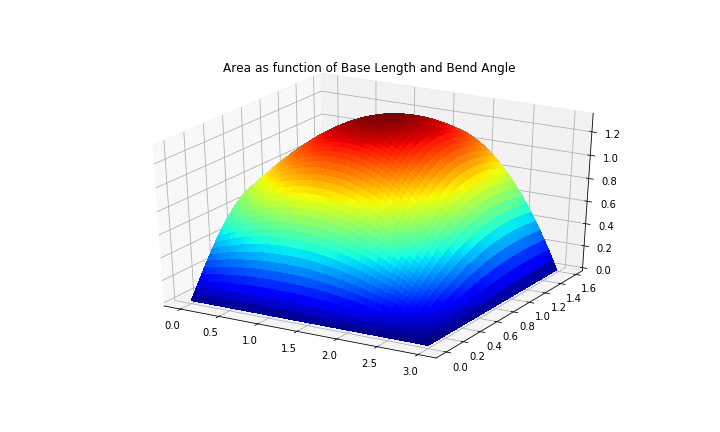
\includegraphics[scale = 0.5]{Channelplot.png}
%\end{figure}

From the plot, we see that there is a maximum that is unique over the domain, achieved when $x^* \approx [1,1]$.

\section*{Analytical Solution}
We attempt to find the exact solution analytically via multivariable calculus. We have the objective  as
%$$A(b,\theta) = \frac{3-b}{2} \sin\theta \big(b + \cos\theta \big)$$
$$\frac{1}{4}(b-3) \sin(\theta) \big((b-3)\cos(\theta) - 2b \big)$$
For which the gradient is 0:
$$ \nabla A(b,\theta) = \bigg(\frac{\partial A}{\partial b}, \frac{\partial A}{\partial \theta} \bigg) = \bigg(\frac{1}{2} \sin \theta \big(3 - 2b - (3-b)\cos \theta),  \frac{3-b}{4} \big (\cos \theta (2b + (3-b)\cos \theta ) - (3-b) \sin^2 \theta \big)  \bigg)$$

Setting the first expression to 0 gives
$$ \frac{1}{2} \sin \theta \big(3 - 2b - (3-b)\cos \theta) = 0 \implies \theta = \pm \arccos \bigg( \frac{2b-3}{b-3} \bigg)$$
And the second to 0 gives 
$$  \frac{3-b}{4} \big (\cos \theta (2b + (3-b)\cos \theta ) - (3-b) \sin^2 \theta \big) =0  \implies b = 3, \ b = -\frac{3\cos^2 \theta - 3 \sin^2 \theta}{2 \cos \theta 	- \cos^2 \theta + \sin ^2 \theta}$$
% \qquad \theta \neq \frac{\pi}{2}(2n + 1) , n \in \mathbb{Z}$$
It is clearly not possible for $b = 3$, so we solve for equivalence of both right-hand expressions. This is given in the appendix. The only solution that falls within the domain is $\theta = \arccos \big(\frac{\sqrt{33} - 3}{6} \big) \approx 1.0957$. This gives $b = \frac{21 - \sqrt{33}}{12} \approx 1.27	13$. This should correspond to the maximum, and can be rigorously proven using the second derivative test.

\section*{Numerical Solution}
The numerical solution is done in Python using gradient descent. 



\section*{Appendix}
\subsection*{Analytical Solution - Finding $\theta$}
\begin{align*}
	\frac{3 - \cos \theta}{2} &= \frac{\sin^2 \theta }{\cos \theta} - \cos \theta \\
	0 &= \frac{1}{2}(3 - \cos \theta ) + \cos \theta  - \frac{\sin^2 \theta}{\cos \theta} \\
	0 &= \frac{\cos \theta (3- \cos \theta)}{2 \cos \theta} + \frac{2\cos^2 \theta }{2\cos \theta} - \frac{2 \sin^2 \theta}{2 \cos \theta }\\
	0 &= 3 \cos \theta + \cos^2 \theta - 2 \sin^2 \theta  \\
		0 &= 3 \cos^2 \theta + 3 \cos \theta. - 2 \\
	\cos\theta &= \frac{-3 \pm \sqrt{33}}{6} \\
	\theta &= \arccos \frac{-3 + \sqrt{33}}{6} + 2 \pi n, \theta = 2\pi - \arccos \frac{-3 + \sqrt{33}}{6} + 2 \pi n; \qquad n \in \mathbb{Z}
	\end{align*}

\end{document}